\section{Les concepts de base:}
Cassandra fournit un schéma de données dynamique afin d'offrir un maximum de flexibilité et de performance. Mais pour bien comprendre cet outil, il faut tout d'abord bien assimiler le vocabulaire de base.

\begin{itemize}[label=\textbullet]
	\item \textbf{Keyspace :} c'est l'équivalent d'une database dans le monde des bases de données relationnelles. À noter qu'il est possible d'avoir plusieurs « Keyspaces » sur un même serveur.
Colonne (Column) : une colonne est composée d'un nom, d'une valeur et d'un timestamp (instant de création).

	\item \textbf{Ligne (Row) :}les colonnes sont regroupées en Rows. Une Row est représentée par une clé et une valeur. Il existe deux types de rows : les « wide row » permettant de stocker énormément de données, avec beaucoup de colonnes et les « skinny row » permettant de stocker peu de données.
	
	\item \textbf{Une famille de colonnes (Column family) :} c'est l'objet principal de données et peut être assimilé à une table dans le monde des bases de données relationnelles. Toutes les rows sont regroupées dans les column family.
\end{itemize}

\begin{figure}[h]
	\centering
    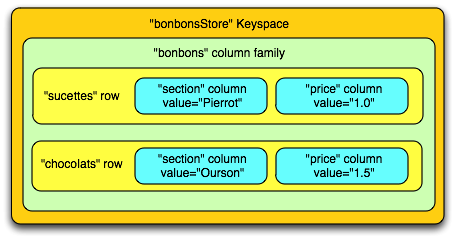
\includegraphics[scale=1]{img/part1/5.1}
    \caption{Les concepts de base}
\end{figure}